\documentclass[]{article}
\usepackage{lmodern}
\usepackage{amssymb,amsmath}
\usepackage{ifxetex,ifluatex}
\usepackage{fixltx2e} % provides \textsubscript
\ifnum 0\ifxetex 1\fi\ifluatex 1\fi=0 % if pdftex
  \usepackage[T1]{fontenc}
  \usepackage[utf8]{inputenc}
\else % if luatex or xelatex
  \ifxetex
    \usepackage{mathspec}
    \usepackage{xltxtra,xunicode}
  \else
    \usepackage{fontspec}
  \fi
  \defaultfontfeatures{Mapping=tex-text,Scale=MatchLowercase}
  \newcommand{\euro}{€}
\fi
% use upquote if available, for straight quotes in verbatim environments
\IfFileExists{upquote.sty}{\usepackage{upquote}}{}
% use microtype if available
\IfFileExists{microtype.sty}{%
\usepackage{microtype}
\UseMicrotypeSet[protrusion]{basicmath} % disable protrusion for tt fonts
}{}
\usepackage[margin=1in]{geometry}
\usepackage{color}
\usepackage{fancyvrb}
\newcommand{\VerbBar}{|}
\newcommand{\VERB}{\Verb[commandchars=\\\{\}]}
\DefineVerbatimEnvironment{Highlighting}{Verbatim}{commandchars=\\\{\}}
% Add ',fontsize=\small' for more characters per line
\usepackage{framed}
\definecolor{shadecolor}{RGB}{248,248,248}
\newenvironment{Shaded}{\begin{snugshade}}{\end{snugshade}}
\newcommand{\KeywordTok}[1]{\textcolor[rgb]{0.13,0.29,0.53}{\textbf{{#1}}}}
\newcommand{\DataTypeTok}[1]{\textcolor[rgb]{0.13,0.29,0.53}{{#1}}}
\newcommand{\DecValTok}[1]{\textcolor[rgb]{0.00,0.00,0.81}{{#1}}}
\newcommand{\BaseNTok}[1]{\textcolor[rgb]{0.00,0.00,0.81}{{#1}}}
\newcommand{\FloatTok}[1]{\textcolor[rgb]{0.00,0.00,0.81}{{#1}}}
\newcommand{\CharTok}[1]{\textcolor[rgb]{0.31,0.60,0.02}{{#1}}}
\newcommand{\StringTok}[1]{\textcolor[rgb]{0.31,0.60,0.02}{{#1}}}
\newcommand{\CommentTok}[1]{\textcolor[rgb]{0.56,0.35,0.01}{\textit{{#1}}}}
\newcommand{\OtherTok}[1]{\textcolor[rgb]{0.56,0.35,0.01}{{#1}}}
\newcommand{\AlertTok}[1]{\textcolor[rgb]{0.94,0.16,0.16}{{#1}}}
\newcommand{\FunctionTok}[1]{\textcolor[rgb]{0.00,0.00,0.00}{{#1}}}
\newcommand{\RegionMarkerTok}[1]{{#1}}
\newcommand{\ErrorTok}[1]{\textbf{{#1}}}
\newcommand{\NormalTok}[1]{{#1}}
\usepackage{graphicx}
\makeatletter
\def\maxwidth{\ifdim\Gin@nat@width>\linewidth\linewidth\else\Gin@nat@width\fi}
\def\maxheight{\ifdim\Gin@nat@height>\textheight\textheight\else\Gin@nat@height\fi}
\makeatother
% Scale images if necessary, so that they will not overflow the page
% margins by default, and it is still possible to overwrite the defaults
% using explicit options in \includegraphics[width, height, ...]{}
\setkeys{Gin}{width=\maxwidth,height=\maxheight,keepaspectratio}
\ifxetex
  \usepackage[setpagesize=false, % page size defined by xetex
              unicode=false, % unicode breaks when used with xetex
              xetex]{hyperref}
\else
  \usepackage[unicode=true]{hyperref}
\fi
\hypersetup{breaklinks=true,
            bookmarks=true,
            pdfauthor={PD Blischak, LS Kubatko and AD Wolfe},
            pdftitle={Example analyses with polyfreqs},
            colorlinks=true,
            citecolor=blue,
            urlcolor=blue,
            linkcolor=magenta,
            pdfborder={0 0 0}}
\urlstyle{same}  % don't use monospace font for urls
\setlength{\parindent}{0pt}
\setlength{\parskip}{6pt plus 2pt minus 1pt}
\setlength{\emergencystretch}{3em}  % prevent overfull lines
\setcounter{secnumdepth}{0}

%%% Change title format to be more compact
\usepackage{titling}
\setlength{\droptitle}{-2em}
  \title{Example analyses with \textbf{polyfreqs}}
  \pretitle{\vspace{\droptitle}\centering\huge}
  \posttitle{\par}
  \author{PD Blischak, LS Kubatko and AD Wolfe}
  \preauthor{\centering\large\emph}
  \postauthor{\par}
  \date{}
  \predate{}\postdate{}




\begin{document}

\maketitle


\section{\texorpdfstring{\emph{Simulation study of population
differentiation}}{Simulation study of population differentiation}}\label{simulation-study-of-population-differentiation}

To study population differentiation we simulated two hypothetical
populations of tetraploids. Sequencing reads were simulated as follows:

\begin{itemize}
\item
  Population 1: allele frequencies were drawn for 2000 loci from a
  Beta(1.25, 1.25) followed by simulated reference and total read data
  for 100 individuals with 15x coverage per locus using the
  \texttt{sim\_reads} function in \textbf{polyfreqs}. The files are
  named \texttt{tot\_reads\_pop1.txt} and \texttt{ref\_reads\_pop1.txt}.
  They are formatted with column headers with a name for each locus
  (loc1, \ldots{}, loc2000) and have row names for each individual
  (ind1, \ldots{}, ind100). This is the format that the data need to be
  in for running through \textbf{polyfreqs}.
\item
  Population 2: same as population 1 but allele frequencies were drawn
  from a Beta(5, 5). The files are named in the same fashion:
  \texttt{tot\_reads\_pop2.txt} and \texttt{ref\_reads\_pop2.txt}.
\end{itemize}

If you wish to re-simulate similar data, use the following code:

\begin{Shaded}
\begin{Highlighting}[]
\CommentTok{# Load polyfreqs}
\KeywordTok{library}\NormalTok{(polyfreqs)}

\CommentTok{# Simulate allele frequencies from the Beta distributions}
\NormalTok{freqs_pop1 <-}\StringTok{ }\KeywordTok{rbeta}\NormalTok{(}\DecValTok{2000}\NormalTok{, }\FloatTok{1.25}\NormalTok{, }\FloatTok{1.25}\NormalTok{)}
\NormalTok{freqs_pop2 <-}\StringTok{ }\KeywordTok{rbeta}\NormalTok{(}\DecValTok{2000}\NormalTok{, }\DecValTok{5}\NormalTok{, }\DecValTok{5}\NormalTok{)}


\CommentTok{# Simulate the read data}
\NormalTok{pop1_dat <-}\StringTok{ }\KeywordTok{sim_reads}\NormalTok{(freqs_pop1, }\DecValTok{100}\NormalTok{, }\DataTypeTok{coverage=}\DecValTok{15}\NormalTok{, }\DataTypeTok{ploidy=}\DecValTok{4}\NormalTok{, }\DataTypeTok{error=}\FloatTok{0.01}\NormalTok{)}
\NormalTok{pop2_dat <-}\StringTok{ }\KeywordTok{sim_reads}\NormalTok{(freqs_pop2, }\DecValTok{100}\NormalTok{, }\DataTypeTok{coverage=}\DecValTok{15}\NormalTok{, }\DataTypeTok{ploidy=}\DecValTok{4}\NormalTok{, }\DataTypeTok{error=}\FloatTok{0.01}\NormalTok{)}
\end{Highlighting}
\end{Shaded}

\begin{Shaded}
\begin{Highlighting}[]
\CommentTok{# Vizualize the difference in the distribution of allelic diversity}
\CommentTok{# btwn pop1 and pop2}
\KeywordTok{plot}\NormalTok{(}\DataTypeTok{x=}\KeywordTok{seq}\NormalTok{(}\DecValTok{0}\NormalTok{, }\DecValTok{1}\NormalTok{, }\DataTypeTok{length=}\DecValTok{1000}\NormalTok{), }\KeywordTok{dbeta}\NormalTok{(}\KeywordTok{seq}\NormalTok{(}\DecValTok{0}\NormalTok{, }\DecValTok{1}\NormalTok{, }\DataTypeTok{length=}\DecValTok{1000}\NormalTok{), }\DecValTok{5}\NormalTok{, }\DecValTok{5}\NormalTok{), }\DataTypeTok{type=}\StringTok{"l"}\NormalTok{, }\DataTypeTok{col=}\StringTok{"red"}\NormalTok{, }\DataTypeTok{ylab=}\StringTok{""}\NormalTok{, }\DataTypeTok{xlab=}\StringTok{""}\NormalTok{, }
     \DataTypeTok{main=}\StringTok{"Distribution of allelic diversity btwn pop1 (blue) and pop2 (red)"}\NormalTok{)}
\KeywordTok{lines}\NormalTok{(}\DataTypeTok{x=}\KeywordTok{seq}\NormalTok{(}\DecValTok{0}\NormalTok{, }\DecValTok{1}\NormalTok{, }\DataTypeTok{length=}\DecValTok{1000}\NormalTok{), }\KeywordTok{dbeta}\NormalTok{(}\KeywordTok{seq}\NormalTok{(}\DecValTok{0}\NormalTok{, }\DecValTok{1}\NormalTok{, }\DataTypeTok{length=}\DecValTok{1000}\NormalTok{), }\FloatTok{1.25}\NormalTok{, }\FloatTok{1.25}\NormalTok{), }\DataTypeTok{col=}\StringTok{"blue"}\NormalTok{)}
\KeywordTok{legend}\NormalTok{(}\DataTypeTok{x=}\StringTok{"topright"}\NormalTok{,}\DataTypeTok{legend=}\KeywordTok{c}\NormalTok{(}\StringTok{"pop1"}\NormalTok{,}\StringTok{"pop2"}\NormalTok{), }\DataTypeTok{col=}\KeywordTok{c}\NormalTok{(}\StringTok{"blue"}\NormalTok{, }\StringTok{"red"}\NormalTok{), }\DataTypeTok{lty=}\DecValTok{1}\NormalTok{)}
\end{Highlighting}
\end{Shaded}

\medskip
\begin{center}
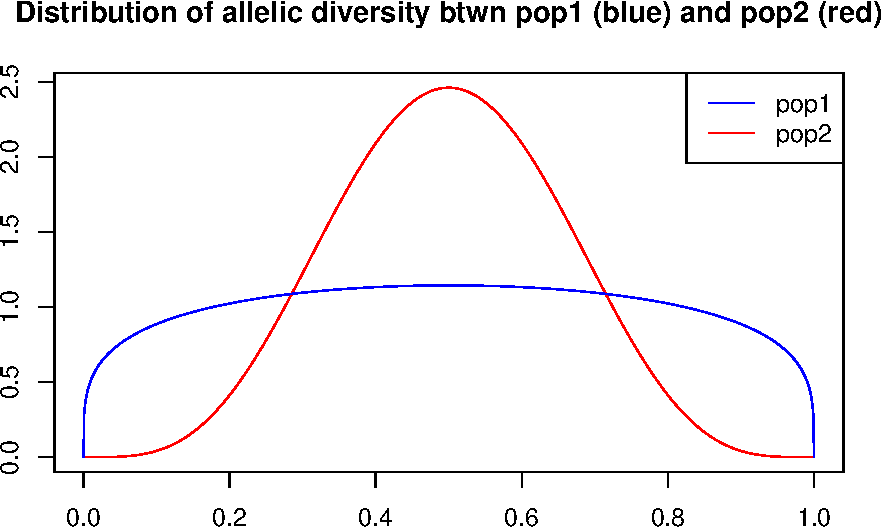
\includegraphics{example-analyses_files/figure-latex/unnamed-chunk-2-1.pdf}
\end{center}
\medskip

Next we will run \textbf{polyfreqs} for population 1. First, we'll read
in the data, convert the tables into matrices and then run them with
\texttt{genotype=TRUE} to get the genotype samples and provide it with a
name for the folder into which the genotype files will be output
(\texttt{geno\_dir="./pop1\_genotypes/"}). It's important that you
remember to specify the directory name in this way (with the \texttt{./}
and \texttt{/}). This tells the program to make the folder in the
current working directory and then to make all new files within that
directory that it created. With 2000 loci and 100 individuals, this
analysis will take some time (on the order of a few hours).

\begin{Shaded}
\begin{Highlighting}[]
\CommentTok{# Read in data using read.table. Remember the row.names and header}
\NormalTok{pop1_tot_table <-}\StringTok{ }\KeywordTok{read.table}\NormalTok{(}\StringTok{"tot_reads_pop1.txt"}\NormalTok{, }\DataTypeTok{row.names=}\DecValTok{1}\NormalTok{, }\DataTypeTok{header=}\NormalTok{T)}
\NormalTok{pop1_ref_table <-}\StringTok{ }\KeywordTok{read.table}\NormalTok{(}\StringTok{"ref_reads_pop1.txt"}\NormalTok{, }\DataTypeTok{row.names=}\DecValTok{1}\NormalTok{, }\DataTypeTok{header=}\NormalTok{T)}

\CommentTok{#Convert the tables to matrices}
\NormalTok{pop1_tot_mat <-}\StringTok{ }\KeywordTok{as.matrix}\NormalTok{(pop1_tot_table)}
\NormalTok{pop1_ref_mat <-}\StringTok{ }\KeywordTok{as.matrix}\NormalTok{(pop1_ref_table)}

\CommentTok{# Run through polyfreqs with genotypes=T}
\CommentTok{# and geno_dir="pop1_genotypes"}
\CommentTok{#}
\CommentTok{# load polyfreqs if you haven'r done so already}
\CommentTok{# library(polyfreqs)}
\KeywordTok{polyfreqs}\NormalTok{(pop1_tot_mat, pop1_ref_mat, }\DataTypeTok{ploidy=}\DecValTok{4}\NormalTok{, }
          \DataTypeTok{iter=}\DecValTok{100000}\NormalTok{, }\DataTypeTok{genotypes=}\NormalTok{T, }\DataTypeTok{geno_dir=}\StringTok{"./pop1_genotypes/"}\NormalTok{, }\DataTypeTok{outfile=}\StringTok{"pop1_mcmc.out"}\NormalTok{)}
\end{Highlighting}
\end{Shaded}

With the analysis for population 1 completed, we can analyze population
2.

\begin{Shaded}
\begin{Highlighting}[]
\CommentTok{# Read in data using read.table. Remember the row.names and header}
\NormalTok{pop2_tot_table <-}\StringTok{ }\KeywordTok{read.table}\NormalTok{(}\StringTok{"tot_reads_pop2.txt"}\NormalTok{, }\DataTypeTok{row.names=}\DecValTok{1}\NormalTok{, }\DataTypeTok{header=}\NormalTok{T)}
\NormalTok{pop2_ref_table <-}\StringTok{ }\KeywordTok{read.table}\NormalTok{(}\StringTok{"ref_reads_pop2.txt"}\NormalTok{, }\DataTypeTok{row.names=}\DecValTok{1}\NormalTok{, }\DataTypeTok{header=}\NormalTok{T)}

\CommentTok{#Convert the tables to matrices}
\NormalTok{pop1_tot_mat <-}\StringTok{ }\KeywordTok{as.matrix}\NormalTok{(pop2_tot_table)}
\NormalTok{pop1_ref_mat <-}\StringTok{ }\KeywordTok{as.matrix}\NormalTok{(pop2_ref_table)}

\CommentTok{# Run through polyfreqs with genotypes=T}
\CommentTok{# and geno_dir="pop2_genotypes"}
\KeywordTok{polyfreqs}\NormalTok{(pop2_tot_mat, pop2_ref_mat, }\DataTypeTok{ploidy=}\DecValTok{4}\NormalTok{, }
          \DataTypeTok{iter=}\DecValTok{100000}\NormalTok{, }\DataTypeTok{genotypes=}\NormalTok{T, }\DataTypeTok{geno_dir=}\StringTok{"./pop2_genotypes/"}\NormalTok{, }\DataTypeTok{outfile=}\StringTok{"pop2_mcmc.out"}\NormalTok{)}
\end{Highlighting}
\end{Shaded}

\subsection{Downstream analyses}\label{downstream-analyses}

With

\section{\texorpdfstring{\emph{Evaluating model adequacy in
autotetraploid potato} (Solanum
tuberosum)}{Evaluating model adequacy in autotetraploid potato (Solanum tuberosum)}}\label{evaluating-model-adequacy-in-autotetraploid-potato-solanum-tuberosum}

\begin{Shaded}
\begin{Highlighting}[]
\CommentTok{# Using autetraploid potato data from the fitTetra package}
\CommentTok{#}
\CommentTok{# If not installed, install it using:}
\CommentTok{# install.packages("fitTetra")}
\CommentTok{#}
\CommentTok{# Then load the data}
\KeywordTok{library}\NormalTok{(fitTetra)}
\KeywordTok{data}\NormalTok{(tetra.potato.SNP)}

\CommentTok{# Get the names of the individuals and loci}
\NormalTok{samples <-}\StringTok{ }\KeywordTok{unique}\NormalTok{(tetra.potato.SNP$SampleName)}
\NormalTok{markers <-}\StringTok{ }\KeywordTok{unique}\NormalTok{(tetra.potato.SNP$MarkerName)}

\CommentTok{# Initialize x and y matrices -- x will be the reference allele}
\NormalTok{potato_mat_x <-}\StringTok{ }\KeywordTok{matrix}\NormalTok{(}\OtherTok{NA}\NormalTok{, }\DataTypeTok{nrow=}\KeywordTok{length}\NormalTok{(}\KeywordTok{unique}\NormalTok{(tetra.potato.SNP$SampleName)), }
                   \DataTypeTok{ncol=}\KeywordTok{length}\NormalTok{(}\KeywordTok{unique}\NormalTok{(tetra.potato.SNP$MarkerName)))}
\KeywordTok{rownames}\NormalTok{(potato_mat_x) <-}\StringTok{ }\NormalTok{samples}
\KeywordTok{colnames}\NormalTok{(potato_mat_x) <-}\StringTok{ }\NormalTok{markers}

\NormalTok{potato_mat_y <-}\StringTok{ }\KeywordTok{matrix}\NormalTok{(}\OtherTok{NA}\NormalTok{, }\DataTypeTok{nrow=}\KeywordTok{length}\NormalTok{(}\KeywordTok{unique}\NormalTok{(tetra.potato.SNP$SampleName)), }
                   \DataTypeTok{ncol=}\KeywordTok{length}\NormalTok{(}\KeywordTok{unique}\NormalTok{(tetra.potato.SNP$MarkerName)))}

\CommentTok{# Get the counts from the data frame}
\NormalTok{for(i in }\DecValTok{1}\NormalTok{:}\KeywordTok{dim}\NormalTok{(potato_mat_x)[}\DecValTok{1}\NormalTok{])\{}
    \NormalTok{tmp <-}\StringTok{ }\KeywordTok{subset}\NormalTok{(tetra.potato.SNP, SampleName==samples[i])}
    \NormalTok{potato_mat_x[i,] <-}\StringTok{ }\NormalTok{tmp$X_Raw}
    \NormalTok{potato_mat_y[i,] <-}\StringTok{ }\NormalTok{tmp$Y_Raw}
\NormalTok{\}}

\CommentTok{# Get the total counts as the sum of x and y and give row and column names}
\NormalTok{potato_mat_tot <-}\StringTok{ }\NormalTok{potato_mat_x +}\StringTok{ }\NormalTok{potato_mat_y}
\KeywordTok{rownames}\NormalTok{(potato_mat_tot) <-}\StringTok{ }\NormalTok{samples}
\KeywordTok{colnames}\NormalTok{(potato_mat_tot) <-}\StringTok{ }\NormalTok{markers}

\CommentTok{# print the tables to file in a format suitable for polyfreqs}
\KeywordTok{write.table}\NormalTok{(potato_mat_x, }\DataTypeTok{file=}\StringTok{"potato_ref_reads.txt"}\NormalTok{,}\DataTypeTok{quote=}\NormalTok{F,}\DataTypeTok{sep=}\StringTok{"}\CharTok{\textbackslash{}t}\StringTok{"}\NormalTok{)}
\KeywordTok{write.table}\NormalTok{(potato_mat_tot, }\DataTypeTok{file=}\StringTok{"potato_tot_reads.txt"}\NormalTok{,}\DataTypeTok{quote=}\NormalTok{F,}\DataTypeTok{sep=}\StringTok{"}\CharTok{\textbackslash{}t}\StringTok{"}\NormalTok{)}
\end{Highlighting}
\end{Shaded}

With the data in the correct format we can go ahead and run
\textbf{polyfreqs}. We will again save the genotypes as we go and will
put them in the folder \texttt{potato\_genotypes/}.

\begin{Shaded}
\begin{Highlighting}[]
\CommentTok{# Read in data using read.table. Remember the row.names and header}
\NormalTok{potato_tot_table <-}\StringTok{ }\KeywordTok{read.table}\NormalTok{(}\StringTok{"potato_tot_reads.txt"}\NormalTok{, }\DataTypeTok{row.names=}\DecValTok{1}\NormalTok{, }\DataTypeTok{header=}\NormalTok{T)}
\NormalTok{potato_ref_table <-}\StringTok{ }\KeywordTok{read.table}\NormalTok{(}\StringTok{"potato_ref_reads.txt"}\NormalTok{, }\DataTypeTok{row.names=}\DecValTok{1}\NormalTok{, }\DataTypeTok{header=}\NormalTok{T)}

\CommentTok{#Convert the tables to matrices}
\NormalTok{potato_tot_mat <-}\StringTok{ }\KeywordTok{as.matrix}\NormalTok{(potato_tot_table)}
\NormalTok{potato_ref_mat <-}\StringTok{ }\KeywordTok{as.matrix}\NormalTok{(potato_ref_table)}

\CommentTok{# Run through polyfreqs with genotypes=T}
\CommentTok{# and geno_dir="./pop2_genotypes/"}
\KeywordTok{polyfreqs}\NormalTok{(potato_tot_mat, potato_ref_mat, }\DataTypeTok{ploidy=}\DecValTok{4}\NormalTok{, }\DataTypeTok{iter=}\DecValTok{100000}\NormalTok{, }
          \DataTypeTok{genotypes=}\NormalTok{T, }\DataTypeTok{geno_dir=}\StringTok{"./potato_genotypes/"}\NormalTok{, }\DataTypeTok{outfile=}\StringTok{"potato_mcmc.out"}\NormalTok{)}
\end{Highlighting}
\end{Shaded}

\end{document}
